\documentclass{article}

\usepackage[margin=1in]{geometry}
\usepackage{graphicx}
\usepackage[doublespacing]{setspace}
\usepackage{booktabs}
\usepackage{xcolor}


\title{Cooperative Driving in Multilane Highway}
\author{Richard Hamilton}
\date{}
\doublespacing
%\linespread{2.0}

\begin{document}


\maketitle
% Chapter 1
\section{Introduction}
%
%This is my citation ~\cite{Plainxml}
%
%\subsection{Background and Motivation}
%fdsfasdf
%
%\subsection{Contributions}
%dfasdfa

%\subsection{Thesis Outline}
%
% Chapter 2
\section{Fundamentals of Autonomous Vehicles}

An autonomous vehicle (AV) is a vehicle that is able to intelligently navigate itself along a trajectory without human intervention, i.e. a vehicle that is capable of performing a steering or speed adjustment task by itself~\cite{Bacha2017}. The Society of Automotive Engineers (SAE) has defined six levels of driving automation known as the SAE J3016, which classifies AVs based on their capabilities and the level of human intervention that is required~\cite{SAE}. The SAE J3016 has become the de facto global standard for stakeholders in the AV technology space. Figure~\ref{fig:autolevel}, outlines the six levels of driving automation from level 0 (no automation) to level 5 (full automation).  As shown in Figure X, one of the specifications for Levels 0 to 2 is that the driver is required to drive or to be engaged at all times even if the driver’s feet are off the pedals and he or she is not steering. Level 1 and Level 2 AVs have features that are able to provide lateral (steering) and longitudinal (brake/acceleration) support to the driver. The two levels differentiate based on the capability to perform lateral and longitudinal control simultaneously; AVs that can provide lateral and longitudinal control simultaneously are considered Level 2, while AVs that can only perform one of these functions at a time are Level 1. Level 2 is the maximum level of automation for commercial AVs in the market today~\cite{Wilko2018}. For a Level 3 AV, the driver is not required to drive or be engaged while the vehicle is in control, however should be ready to take control of the vehicle when requested in difficult situations. Level 4 and Level 5 AVs do not require the driver to take over driving in any situation, rendering them fully automated vehicles. AVs are classified as Level 4 when they are fully autonomous (no driver required) but only in controlled areas, whereas Level  5 is reserved only for vehicles that are fully autonomous under all situations everywhere.

% figure of sae levels of automation
\begin{figure}[htbp]
\begin{center}
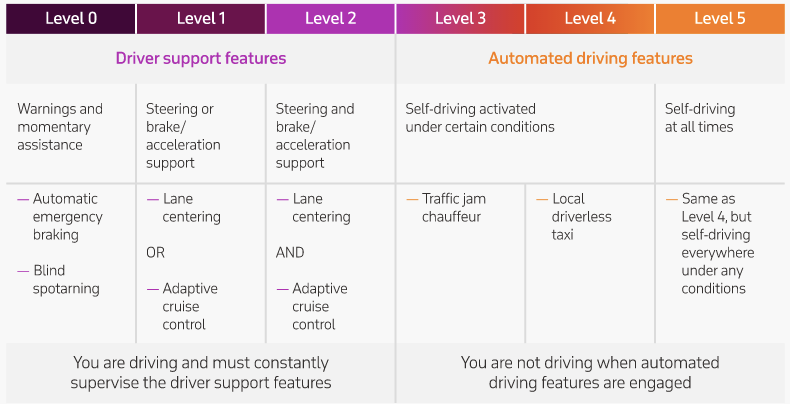
\includegraphics[scale=0.6]{figures/sae_levels_of_auto.png}
\caption{SAE J3016 six levels of autonmation~\cite{AVSensors}}
\label{fig:autolevel}
\end{center}
\end{figure}

AV systems are considered to possess artificial intelligence (AI) capabilities, which is the ability for a machine to simulate intelligent human tasks~\cite{Malcolm1994}. Intelligent human tasks include: 1) Perception: translating external information into an internal representation, 2) Cognition: manipulating and processing internal information to derive new signals, and 3) Execution: converting signals into action. As illustrated in the general architecture of AV systems in Figure~\ref{fig:av_arch}, AV systems generally perform all three tasks ~\cite{Naoki2014}.

AV systems should be able to determine where the vehicle is located and what objects are around it, both of which are achieved with the use of powerful sensors during Perception~\cite{Naoki2014}. Sensors are used to perceive key information such as -- but not limited to -- distance, speed and classification of traffic objects from the vehicle’s surroundings.  Once sensors receive information from the surroundings, dedicated computing modules process the information to derive control signals during Cognition (Control). Before computing a control signal, some AV systems may also be required to make high level control decisions (decision making) and/or determine a reference trajectory (path planning). High level control decisions may include lateral lane change in both directions, speeding up, speeding down, idling, and others. Finally AV systems use computing modules and mechanical systems to execute control signals, during execution~\cite{Naoki2014}.

% figure of av architecture
\begin{figure}[htbp]
\begin{center}
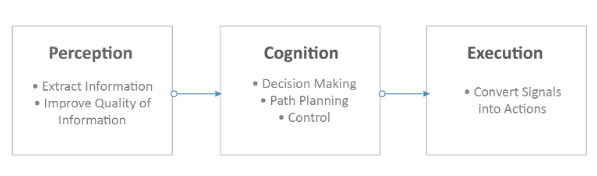
\includegraphics[scale=0.7]{figures/av_architecture.png}
\caption{AV systems architecture base on intelligent tasks.}
\label{fig:av_arch}
\end{center}
\end{figure}
	
	The remainder of this chapter discusses sensors, computing modules, and mechanical systems relating to perception, cognition and execution.

\subsection{Perception}

The goal of perception in AV systems is to extract required information about the vehicle and its environment in order to navigate successfully~\cite{Naoki2014}.  In general, perception is achieved by using sensors to measure or capture information from the environment and subsequently post processing sensor data to a) extract relevant information and b) improve the quality of the information. This ability to perform perception successfully is what affords AVs the capability to make intelligent decisions in real time. Moreover, advanced technologies such as vehicle-to-everything (V2X) allow high level perception in which vehicles have the capability to communicate with traffic systems in their surroundings, including other vehicles. Given the unique perception capabilities of V2X technologies and the relevance to this research, more information about V2X is provided separately in Section 2.4.

\subsubsection{Sensing}

AVs require the ability to perceive the environment surrounding the vehicle and also measure values within the system, tasks that are achieved by  its sensors~\cite{Naoki2014}. Sensors have to be able to create a perspective and localizational view of the environment quickly and accurately to produce a high quality understanding of what situation the vehicle is in. There are two types of sensors used in AVs: 1) exteroceptive sensors, which are used to perceive and extract information about the environment surrounding the vehicle and 2) proprioceptive sensors, which measure values from within the system such as motor speed, vehicle position, etc.~\cite{Campbell2018}.

\textbf{Exteroceptive Sensors}

Four exteroceptive sensors that are commonly used in AVs, namely LiDAR, radar, camera and ultrasonic sensors are discussed in detail below.

1) \emph{LiDARs} (Light Detection and Ranging) are active electromagnetic sensors used for measuring distance and creating 3D representations of an AV’s surrounding environment~\cite{Campbell2018}. LiDARs emit laser or light outwards and measure the time it takes for signals to be reflected back to the sensor, a principle known as “time of flight” (TOF).TOF and the speed of the signal -- which in the case of LiDARs is the speed of light -- are used to calculate the distance of objects detected. LiDARs today can make distance measurements at rates higher than 150 kilohertz (150,000 pulses per second). LiDARS have a range of over 250m and are therefore classified as  long-range sensors. LiDARs provide major advantages in AV systems due to their  precision, accuracy, and high resolution. However, drawbacks of LiDARs include costliness and low availability. Given the advantages that LiDARs provide, a plethora of current research aims to address their drawbacks, including the development of solid-state LiDARs and infrared LiDARs for widespread usage.

2) \emph{Radars} are electromagnetic sensors that emit radio waves to measure distance, angle and velocity of objects~\cite{Campbell2018}. Radars can be used in multiple frequency bands (24 GHZ, 77 GHz, etc.); the higher the frequency, the higher the ability for the sensor to distinguish between multiple objects. Classes of radars include short, medium and long range and individual classes cover a subset of ranges between 50m to 150m and over. One of the greatest advantages of using radars is their robustness towards all kinds of environmental conditions -- such as rain, night etc. Additionally, in contrast to LiDARs, radars are significantly less expensive and in general more readily available.

3) \emph{Cameras} are a type of passive exteroceptive sensor which means that unlike the aforementioned sensors, cameras do not emit their own signals. Instead, cameras  use ambient light to produce a digital 2D representation of a 3D environment~\cite{RMLAV}. One significant advantage of using cameras is their ability to perceive colours and textures, which is extremely beneficial when identifying objects in the environment such as road signs, traffic lights, lane markings, etc.[Campbell2018]. While images from cameras can be used to compute distance to objects, this requires complex algorithms and most times also a stereo vision set up, in which cameras with two or more separate lenses each produce separate images. One disadvantage to cameras as sensors in AV systems is that their performance is adversely affected by low intensity light and adverse weather conditions, as a result making them only reliable appropriate conditions.

4) \emph{Ultrasonic sensors} are sonar based sensors that emit sound waves to measure the distance of objects~\cite{Campbell2018}. Similar to other active sensors, ultrasonics use the TOF principle to compute distances to detected objects. Major advantages to using ultrasonic sensors include their cost-effectiveness as well as their robustness towards adverse and changing weather conditions. While these are excellent benefits, ultrasonic sensors come with their own set of drawbacks. While measuring distances to objects in close proximity yields best results using ultrasonics, their accuracy depletes with increasing distances given that disturbances in sound waves increase with distance. Ultrasonic sensors are typically used in ranges from 15cm to 11m~\cite{USonics}.

Majority of today's automotive original equipment manufacturers (OEMs) typically use LiDARs, radars and cameras for exteroceptive sensors in AVs~\cite{AVSensors}. Figurex shows the common locations for such sensors on an AV and also the location of computing modules.


% figure of sensor locations
\begin{figure}[htbp]
\begin{center}
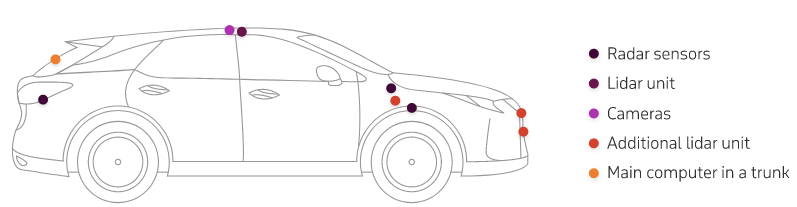
\includegraphics[scale=0.5]{figures/sensor_locations.png}
\caption{Typical location of exteroceptive sensors on AVs~\cite{AVSensors}.}
\label{fig:av_arch}
\end{center}
\end{figure}

\textbf{Proprioceptive Sensors}

Three proprioceptive sensors that are commonly used in AVs, namely global positioning system, inertial measurement units, and encoders are discussed in detail below.

1) \emph{Global Positioning System (GPS)} is a navigation system that uses satellite data, receiver input and algorithms to synchronize the location, velocity and time data for air, sea, and land travel~\cite{Campbell2018}. GPS technology is commonly found in vehicles of all types today. Just as in non-autonomous vehicles, AVs use GPS for navigation and localization purposes. While GPS has become a very commonplace navigation tool, one significant disadvantage of using GPS for localization is that there are many factors that can diminish its accuracy. For example, GPS requires an unobstructed line of sight between satellites and receivers, but signals can easily be obstructed due to objects in the environment including high buildings, trees, tunnels, etc.

2) \emph{Inertial Measurement Unit (IMU)} is an electronic device that is composed of accelerometers, gyroscopes and magnetometers to measure an object’s acceleration, angular rate and magnetic field, respectively~\cite{Campbell2018}. The aforementioned measurements are calculated for each of the orthogonal X, Y, and Z axes.  IMU provides valuable information about the AV’s orientation in space. One setback of   IMU sensors is that they are only  capable of providing information about orientation and dynamics of the vehicle and are unable to provide actual positional information. Another disadvantage of IMUs is that the gyroscope measurement of the current angle is an estimation by integrating the measured angular rotation, this estimation induces errors which can be compounded; this is known as drift error. A common solution to overcome this drawback is to use GPS to correct for drift errors.

3) \emph{Encoders} are electronic devices used to convert linear or angular position to an analog or digital signal [Campbell2018]. Encoders are typically used to provide odometer data on the vehicle. Another interesting application of encoders is called dead reckoning, a process in which the encoder is attached to one of the wheels  to approximate the relative position travelled,based on measured distance, from a known starting point. Dead reckoning is a common solution to estimate a vehicle's position when GPS signal is lost.

\subsubsection{Sensing Post-Processing} 

In general raw data from sensors are not immediately useful and consequently requires post processing to filter and improve accuracy of the data. Below four common post processing algorithms -- object detection, lane detection, localization and mapping, and sensor fusion -- are discussed in detail.

1) \emph{Object Detection}: Object detection is the computer vision process of detecting and classifying instances of objects of a certain class with an image, such as traffic signs, lane markings, vehicles, etc.~\cite{Liu2021}. Object Detection is an important task in AV systems application given that different classes of objects warrant different actions. Generally speaking, over the course of time and development in this field, object detection has evolved from conventional techniques to deep learning techniques . Conventional techniques -- algorithms are developed manually -- include paradigms such as Histogram of Oriented Gradients (HOG) feature descriptor, and Deformable Part-based Model (DPM)  [Liu2021]. Although many of today’s most advanced methods far outperform object detection via conventional techniques, many current algorithms are still influenced by their contributions including hybrid models and bounding box regression. Deep learning based object detection techniques are algorithms that automatically learn models of object detection using neural networks . Examples of the state-of-the-art methods that use deep learning techniques include the Regions of CNN features (RCNN) series, Single Shot MultiBox Detector (SSD) series, and You Only Look Once (YOLO) series ~\cite{Liu2021}. 

2) \emph{Lane Detection}: Lane detection is a special type of object detection that involves detecting lanes on a road using input from a camera~\cite{Liu2021}. Performing lane detection is a pivotal function of AV systems, because it enables AVs to drive within their lanes, correctly avoid collisions, and also perform subsequent decision making and path planning tasks. Traditional lane detection techniques rely on cues such as colour-based features combined with Hough transform and Kalman filters to detect lane markings~\cite{Liu2021}. The performance of these traditional techniques, however, varies with road scene variations consequently making it difficult to achieve reasonable accuracy. Recently, deep learning-based approaches have provided more accurate and faster performance in the lane detection field. For instance, a Vanishing Point Guided Network (VPGNet), which is an end-to-end deep Convolutional Neural Network (CNN) that can simultaneously detect road markings and lanes lines, introduces vanishing point prediction task into the network which improved the accuracy of detection even in some bad situations such as rainy days or at night~\cite{Lee2017}.

3) \emph{Localization and Mapping}: Localization is the process of finding the ego vehicle’s-position relative to a map, and its accuracy affects the feasibility and safety of navigation and path planning~\cite{Dhongade2019}. Currently, GPS-IMU based localization is widely used for automated highway driving, however, the accuracy required for urban automated driving cannot be fulfilled by GPS-IMU systems. One practical solution is the use of pre-build high definition (HD) maps, which are maps containing geographic details that are not normally present on traditional maps, such as road and lane information~\cite{Daruthep2020}. Data for HD maps are collected from Mobile Mapping System (MSS) which are typically vehicles equipped with mapping sensors, navigation sensors, control units and vehicle mounted cameras. The raw data then gets processed to organize input and output data in a sensible way, as well as generate search-able indexes for all data -- allowing the system to handle large amounts of data. AVs can access information from HD Maps stored onboard the vehicle to achieve accurate lane level localization.

4) \emph{Sensor Fusion}: The goal of perception is to accurately sense the surrounding environment~\cite{Liu2021}. Fusing the data from multiple sensor types creates a more reliable system as it significantly increases precision and accuracy.  In sensor fusion, a suite of sensors provide specific information about the same environment scene; this information is then combined from all sources,  ultimately yielding higher quality output. As described previously, sensors of different types come with their own set of strengths and weaknesses; leveraging and fusing the strengths of each individual sensor ultimately results in the best performance. For example, cameras provide excellent color and texture information, which is significant for object classification, however  cameras are less adept at performing accurate distance estimation with images due to the loss  of information from reduced dimension. On the other hand, radars and LiDARs provide little to no information regarding color or texture but are highly proficient at actively providing spatial measurements that yield accurate distance estimation. In order to obtain a more accurate and complete picture of the vehicle’s environment, AVs combine information from different sensors in a way that emphasizes and leverages their strengths.Table~\ref{tab:sensorfusion} shows common sensor fusions used in AVs.

\begin{table}[htbp]
\caption{Typical sensor fusion used for AV applications.}
\begin{center}
\begin{tabular}{|l|p{2in}|p{2.5in}|}
\hline
\textbf{Sensor Types} & \textbf{Objectivive} & \textbf{Sensor Information Extraction} \\
\hline
Vision - LiDAR/Radar & Localization, classification and distance and velocity measurement & Camera $\rightarrow$ classification

Distance measure $\rightarrow$ LiDAR/Radar

Velocity measurement $\rightarrow$ Radar \\
\hline
GPS-IMU & Absolute localization & GPS $\rightarrow$ localization (unobstructive)

IMU $\rightarrow$ dead reckoning \\
\hline
GPS-Encoder & Absolute localization & GPS $\rightarrow$ localization (unobstructive)

Encoder $\rightarrow$ dead reckoning \\
\hline
\end{tabular}
\end{center}
\label{tab:sensorfusion}
\end{table}

\subsection{Cognition}

The goal of cognition in AV systems is to receive information from the surroundings using any of the above mentioned perception techniques, and process this information to derive control signals~\cite{Naoki2014}. 

\subsubsection{Decision Making}

Advanced AV systems are required to make decisions similar to how human drivers do\cite{Wang2021}. Generally, decisions include behaviours such as left lane change, right lane change, speeding up, speeding down or idling. While these decision making capabilities are present in AVs,  deriving accurate, efficient and safe decisions in complex environments can still be a significant challenge. Decision making is based on various factors including traffic rules, surrounding environmental conditions, and the dynamic state of the vehicle. Currently, two main paradigms exist for decision making: 1) rule based method and 2) machine learning based method [Wang2021]. The rule based method establishes a behaviour rule library according to information such as driving rules, knowledge, experience and traffic rules, and subsequently converts the vehicle states into logic rules corresponding to driving behaviours. The downside of using rule based methods is that at any given point, a vehicle can be in a number of vehicle states, making it difficult to implement a rule library that has coverage for all states. Machine learning (ML) methods provide an alternative to rule based methods through its ability to autonomously generate a driving algorithm by learning what actions to take given different traffic situations. Common ML techniques that perform decision making include deep learning methods (DNN), reinforcement learning (RL) and recurrent neural networks (RNN).

\subsubsection{Path Planning}

Path planning is the process of computing a reference trajectory approaching the vehicle’s destination that the vehicle can safely navigate~\cite{Ma2012}. Path planning is a complex process because not only does the trajectory have to be within driveable regions, it also has to obey the laws of the lane and rules between other vehicles for a collision-free path.  Similar to decision making, not all AV systems have path planning capabilities. More specifically, only AV systems that have lateral control -- in which the driver is not required to steer when the AV system is in control -- tend to have path planning algorithms~\cite{Wang2021}. Path planning consists of two types of planners, a high level planner and a low level planner, both of which have their own particular functionality. The high level planner selects the optimal path from a digital map like a car navigation system while the low level planner generates a trajectory at a lane and sublane level which the AV finally follows~\cite{Naoki2014}.

\subsubsection{Control}


\subsection{Execution}

The goal of execution in AV systems is to convert signals derived during cognition into actions~\cite{Naoki2014}. In general, lateral and longitudinal control requests are achieved by the steering system and propulsion system of the AV, respectively. The steering system changes the orientation of the front wheel, which results in the change of the heading of the vehicle, ultimately  changing the lateral position of the vehicle. On the other hand, commands related to longitudinal control are executed by the propulsion system, which includes the braking system. Using the propulsion system, actions to change the velocity of the vehicle can be executed.

% Chapter 3

\section{Advance Driver Assistance Systems}

The function of Advanced Driver Assistance Systems (ADAS) is to prevent vehicle collisions either actively or passively. Active control involves taking full or partial control of the vehicle’s functionality, whereas passive control involves alerting the driver of unsafe situations via audio or visual information, so that the driver can mitigate a collision~\cite{Emre2012}. Due to the consequences posed by  vehicle collisions, fuel economy and congestion, ADAS has become a central focus of research in this field. Advantages of ADAS include that it allows  for enhanced driving comfort, improved safety, improved traffic capacity and reduced fuel consumption. Before the era of high penetration of AVs in the market, driver assistance systems such as ADAS are the precursors that deliver safety benefits to users~\cite{Utriainen2020}. The remainder of this section will discuss active ADAS features including automatic emergency braking, adaptive cruise control, cooperative adaptive cruise control, lane keep assist and lane centering control  in detail.

\subsection{Automatic Emergency Braking}

Automatic emergency braking (AEB) is an active safety system that activates a vehicle’s braking system when a potential collision is detected. Vehicles that are equipped with AEB have two components competing for control over the vehicle: 1) the human driver and 2) the AEB control. Both controllers’ objective is to avoid a collision with objects in its path. According to experimental analysis, under normal situations, the time interval between the perception of an object to the initiation of a controlled action to avoid a collision for the average human driver is in the order of seconds~\cite{Amimi2017}, which can in some situations be too much latency to avoid an imminent collision. AEB systems can reduce the number of forward traffic collisions.


In non-autonomous  passenger vehicles, the human driver has three mechanical control inputs, namely the gas pedal, brake pedal and steering wheel, which control acceleration, deceleration and steering, respectively~\cite{Amimi2017}. The strength of the three driver inputs are measured by an Electronic Control System (ECS) that forms 3D control variables to determine the current intention of the driver. The ECS also evaluates the practicality of the driver’s intention based on physical laws and safety of the vehicle, and makes modifications in the event of violations~\cite{Amimi2017}.

In AEB control, the laser scanner and camera, which form a vital part of an AEB architecture, retrieve information and direct it to the sensor fusion unit, to perceive accuration information about the vehicle’s environment. The AEB control unit uses accident aversion logic to assess the criticality of the scenario and determine the brake point -- vehicle’s deceleration -- to avoid collision. AEB uses this information in addition to information from the ECS about the driver's intention to determine if to activate AEB and if so determine the brake request to meet the computed brake point~\cite{Amimi2017}.


\subsection{Adaptive Cruise Control}

Adaptive cruise control (ACC) is an ADAS feature that automatically maintains a steady desired speed while keeping a set time gap to the leading vehicle~\cite{Lingyun2010}. While ACC is considered an extension of Conventional Cruise Control (CCC), it actually incorporates two modes: 1) the CCC mode, which allows a vehicle to travel at a desired speed set by the driver, and 2) the headway control mode, which allows the vehicle to maintain a safe distance from a preceding vehicle by adjusting its speed~\cite{Lingyun2010}. If a preceding vehicle is not present, ACC will operate in the CCC mode only. If a preceding vehicle is present close to the ego vehicle or travelling slowly ahead, ACC will shift and operate in the headway control mode. Distance and relative speed information of preceding vehicles used by ACC systems is provided by onboard range sensors (such as radar, LiDAR or camera). In the first generation of ACC systems, long range radar (LRR) and LiDAR sensors were commonly used. To improve the safety and usage rate of ACC systems, mid- and short-range radars were included in subsequent generations. 


A key part to the design of any ACC system is the type of spacing policy implemented. Three common spacing policies are constant distance, constant time headway, and constant safety factor spacing, which are summarized in table~\ref{tab:spacingpolicy}~\cite{Wu2020}. Today, constant time headway is the most common spacing policy used by automakers due to their  feasibility, traffic flow stability, safety, capability and reliability.

\begin{table}[htbp]
\caption{Three common spacing policies used in ACC systems.}
\begin{center}
\begin{tabular}{|l|p{2.5in}|}
\hline
\textbf{Spacing Policy} & \textbf{Description} \\
\hline
Constant distance & Fixed gap between host and lead vehicle, independent from the velocity. \\
\hline
Constant time headway & Desired following distance is proportional to the speed of the vehicle. \\
\hline
Constant safety factor spacing & Following distance is determined by safe stopping distance and proportional to a safety factor. \\
\hline
\end{tabular}
\end{center}
\label{tab:spacingpolicy}
\end{table}

\subsection{Cooperative Adaptive Cruise Control}

One of the most promising technologies of CAVs, vehicles with V2X technologies that are able to connect to external traffic systems, is cooperative adaptive cruise control (CACC). CACC is an extension of ACC with the added element of cooperative speed control~\cite{Wang2018}. CACC systems use shared information from other CAVs in a network via V2V technology. With shared information such as acceleration, speed and position, CACC systems have the capability to orchestrate platooning, a cooperative driving application where autonomous and semi-autonomous vehicles move in a train-like manner by keeping constant distance between vehicles.  Additionally, CACC systems can allow vehicles to be driven at harmonized speeds with shorter time headways between CAVs. These features result in vehicles being tightly coupled together, which results in the increase of roadway capacity leading to decreased congestion. The most widely adopted design for CACC application is called the distributed consensus strategy. The consensus strategy contains a network of agents (CAVs) that collectively reach an agreement on a certain state, in this case velocity, -- of all agents. “Distributed” in distributed consensus strategy refers to how a network of agents come to a consensus, in that vehicles in a platoon only communicate with its following vehicle to reach a consensus for the whole platoon instead of a centralized scheme in which all vehicles communicate with each other in a network. The distributed consensus strategy has multiple advantages including 1) String stability parameter errors are attenuated along upstream direction and 2) platoon size is not limited by communication range. While proposed CACC control strategies have been proven mathematically and analyzed in theory, only few have been implemented and tested in real world situations~\cite{Wang2018}.

\subsection{Lane Keeping Assistance}

LKA is another ADAS feature that automatically detects lane markings on the road to actively steer the vehicle back into its lane with a slight steering torque in the event of lane drifting~\cite{Utriainen2020}. Between 2015-2017, departures from lanes were the cause of 52\% of fatal traffic accidents in the US~\cite{Cumali2019}. Therefore, ADAS features that prevent vehicles from drifting outside their lane can significantly help reduce fatal accidents. In LKA systems, perception is achieved by 1) extracting lane lines and road boundaries related information such as lane width, lane number, and roadway curvature, and 2) assessing the current state of the ego vehicle’s dynamics. Sensor technologies currently used to extract lane and road information includes cameras, radars, sonars and LiDARs, or high definition maps. Lane detection data may be augmented by information from connected data sources such as GPS data, HD Maps and V2X for localization and safety purposes. LKA systems process information received via perception to localize the vehicle relative to its lane and determine torque command required to keep the vehicle from drifting~\cite{Lei2006}. Next, the steering system arbitrates the torque request with steering input from the driver to orient the vehicle’s front wheels to adjust the vehicle’s heading.

\subsection{Automated Lane Centering}

LCC is an automated lane centering system that provides automatic lateral control~\cite{Cumali2019}. It is important to distinguish LCC from LKA; while LKA aims to nudge a vehicle back into its lane upon drifting, LCC aims to maintain a central position of the vehicle within a lane. The perception design of LCC is similar to that of LKA, where lane and road information is extracted from an onboard camera and distance measuring sensors. However, unlike LKA, LCC requires a path planning function that  computes a reference trajectory in the lane travelled by the vehicle~\cite{Cumali2019}. The reference trajectory is an imaginary desired path which may be in the center of the lane or offset from the center of the lane. For example, the reference trajectory may be closer to the inner lane markings when traveling along a curve. LCC control determines the corrective adjustment the vehicle should make by computing the vehicle’s headway error, defined as the offset of the vehicle’s heading relative to the reference trajectory. LCC control algorithm uses the headway error to determine the  torque request required to make the adjustment to minimize headway error. Similar to LKA, the torque request gets sent to the steering system to orient the vehicle’s front wheels to adjust the vehicle’s heading accordingly.

% Chapter 4
\section{Modelling and Simulation of Autonomous Vehicle}

The high expenditure, infrastructure and risk associated with the development of real scale models of AV place limitations on the ability to test AV on the road~\cite{Araujo2016}. A low cost alternative, as a preceding verification step, would be to use  simulated vehicle models to study dynamic responses of such AVs’ components. Simulational verification can have several advantages, besides the decreased expenditure, including the optimization of the product development flow, lower risk of injuries, failure prediction, design and concept gap assessment and so on. However, simulations have limitations, such as, they are inherently approximations of the real world scenarios, which might lead to uncertainties in some cases~\cite{Traub2016}. Nevertheless, if used appropriately and the limitations of the models used in the simulation are known, they can be a very valuable medium. Furthermore, this can be especially useful with newer technological innovations such as in the field of AV technology. 

This section provides an overview of the major building blocks associated with the development of an autonomous capable model in a virtual simulation environment, as shown in Figure~\ref{fig:avmodelling}, as well as a review of the relevant literature. The subsystems that are vital in simulations of AVs include the driving environment model, sensor model, and ADAS Control Model, discussed in detail next.

% figure of AV modelling overview
\begin{figure}[htbp]
\begin{center}
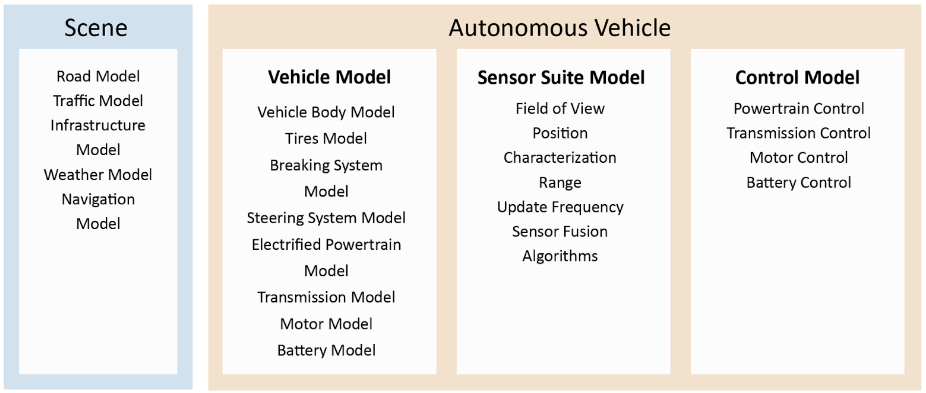
\includegraphics[scale=0.5]{figures/avmodel.png}
\caption{Components of an AV's virtual simulation model.~\cite{Hamilton2018}.}
\label{fig:avmodelling}
\end{center}
\end{figure}



\subsection{Driving Scene Model}

The driving scene model of AV virtual simulation includes environmental objects and elements such as roads, traffic, infrastructure, weather, navigation constraints, etc. In simulation software, road networks can be customized with different lengths, gradients and intersections, according to the needs of the user~\cite{Amimi2017}. Some software also allows the user to model real road networks by using  third-party software such as Google Maps~\cite{Olofsson2015}. Full topographical road network models can also be generated using surveying methods, which involve capturing a road network using cameras and sensors.~\cite{Wellington2006} describes a method for simulating off-road terrain which may contain variations in local terrain height due to vegetation and obscured obstacles.
 
Another important driving scene element involved in simulations is traffic, a vital component in AV simulations given that AVs will interact with their surrounding traffic. Majority of modeling software allows automatic traffic generation by specifying features such as traffic density and direction. Additionally, they enable the control of individual vehicles in order to create customized traffic scenarios~\cite{Olofsson2015}. Traffic can be modeled from microscopic, macroscopic, or micro-macroscopic levels. Microscopic modeling focuses on individual vehicle decisions and their effects on traffic; microscopic modeling is useful for modeling real life drivers~\cite{Xu2011}. Macroscopic modeling focuses on aggregate behavior, and is useful for simulating traffic flow, such as freeway flow.
 
Weather conditions are also an important environmental factor that should be captured in ADAS simulations. Weather conditions not only have an impact on the AV’s sensors, but also the dynamic behaviour of the vehicle such as drag from wind~\cite{Amimi2017}.~\cite{Praveen2017} describes a simulation model for fog, rain, and windshield effects.


\subsection{Perception Modelling}

\subsection{Cognition Modelling}

\subsection{Execution Modelling}
%
%% Chapter 5
%\section{Machine Learning in Autonomous Vehicles}
%
%\subsection{Types of Machine Learning}
%
%\subsection{Machine Learning in Perception}
%
%\subsection{Machine Learning in Cognition}
%
%%Chapter 6
%\section{Deep Q-Learning}
%
%\subsection{Reinforcement Learning}
%\subsubsection{Elements of Reinforcement Learning}
%\subsubsection{Exploration vs Exploitation}
%
%\subsection{Types of Reinforcement Learnign}
%\subsubsection{Q-Learning}
%\subsubsection{Deep Q-Learning}
%
%%Chapter 7
%\section{Experimental Setup}
%
%\subsection{Deep Q-Learning Cooperative Automated Driving Rerun}
%
%\subsection{Deep Q-Learning Cooperative Automated Driving Revise}
%
%\subsection{Deep Q-Learning Cooperative Automated Driving with Second Perception Field Input Features}
%
%% Chapter 8
%\section{Results and Discussions}
%
%% Chapter 9
%\section{Conclusions}

\bibliographystyle{IEEEtran}
\bibliography{Thesis}

\end{document}